\section{\epsolute{}: Efficiently Querying Databases While Providing Differential Privacy~\cite{epsolute}}

	\begin{frame}[label={frame:epsolute-motivation}]

		\frametitle{Motivation}

		\begin{block}{The problem}

			\begin{itemize}
				\item<1-> Previous solutions work in the snapshot model (adversary steals the hard drive)
				\item<1->
					What about \textbf{persistent} adversary (malicious script with \texttt{root} permissions)? \\
					\begin{small}
						\indent{} Model: \alert{persistent}, query type: \alert{point} and \alert{range}
					\end{small}
				\item<1-> Need to protect \alert{access pattern} and \alert{communication volume}
				\item<2->
					Using ORAM to hide the access pattern \\
					\begin{small}
						\indent{} Expensive, each request costs $\bigO{\log n}$ \hyperlink{frame:appendix:oram}{\beamerskipbutton{ORAM definition}}
					\end{small}
				\item<3->
					Adding fake records (noise) to the answer to hide the result size \\
					\begin{small}
						\indent{} How much noise to add to have a guarantee and the least overhead? \\
						\indent{} Adding a constant or a uniformly sampled noise is not an option \\
						\indent{} Differential Privacy!
					\end{small}
			\end{itemize}

		\end{block}

	\end{frame}

	\begin{frame}{Differential Privacy, LPA and Sanitation}

		\begin{definition}[\alert{Differential Privacy}, adapted from~\cite{our-data-ourselves, differential-privacy-original}]
			\justify%

			A randomized algorithm \algo{A} is $(\epsilon, \delta)$-differentially private if for all $\database_1 \sim \database_2 \in \searchKeyDomain^\dataSize$, and for all subsets $\mathcal{O}$ of the output space of \algo{A},
			\[
				\probability{ \algo{A}{ \database_1 } \in \mathcal{O} } \leq \exp(\epsilon) \cdot \probability{ \algo{A}{ \database_2 } \in \mathcal{O} } + \delta \; .
			\]
		\end{definition}

		\pause%

		\begin{columns}[T,onlytextwidth]
			\column{0.6\textwidth}

				\begin{block}{How to make sense of it?}
					\begin{itemize}
						\item<2->
							Differential Privacy is a property of an algorithm \\
							\begin{small}
								\indent{} What about $\epsilon$ and $\delta$?
							\end{small}
						\item<3->
							How to construct such an algorithm? \\
							\begin{small}
								\indent{} Laplace Perturbation Method!
							\end{small}
						\item<4->
							What if negative value is sampled? \\
							\begin{small}
								\indent{} Cannot truncate one side, must shift entire distribution
							\end{small}
					\end{itemize}
				\end{block}

			\column{0.4\textwidth}

				\centering
				\visible<5->{
					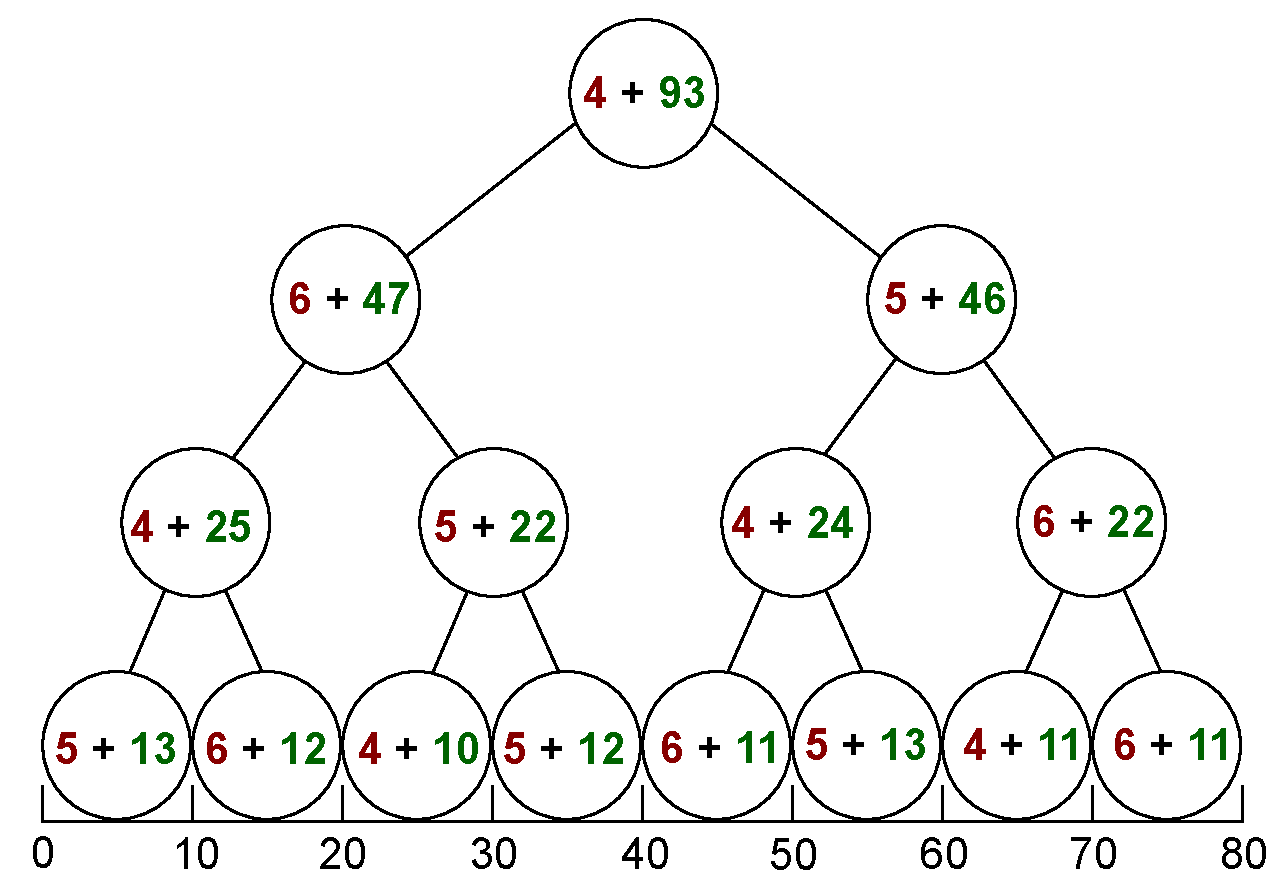
\includegraphics[width=1.0\linewidth]{sanitizer}
				}

		\end{columns}

	\end{frame}

	\begin{frame}{Differentially Private Outsourced Database System}

		\begin{definition}[\alert{Computationally Differentially Private Outsourced Database System}]
			\justify%

			We say that an outsourced database system \protocol{} is $(\epsilon, \delta)$-computationally differentially private (a.k.a.~CDP-ODB) if for every polynomial time distinguishing adversary \adversary{}, for every neighboring databases $\database \sim \database^\prime$, and for every query sequence $\fromNtoM{\query}{1}{m} \in \querySet^m$ where $m = \mathsf{poly}(\lambda)$,

			\begin{multline*}
				\probability{\adversary \left( 1^\lambda, \view{\protocol, \server}{\database, \fromNtoM{\query}{1}{m}} \right) = 1 } \leq \\
				\exp{\epsilon} \cdot \probability{\adversary \left( 1^\lambda, \view{\protocol ,\server}{\database^\prime, \fromNtoM{\query}{1}{m}} \right) = 1} + \delta + \negl \; ,
			\end{multline*}
			the probability is over the randomness of the distinguishing adversary \adversary{} and the protocol \protocol{}.
		\end{definition}

		\pause%

		Note:
		\begin{itemize}
			\item Entire view of the adversary is DP-protected
			\item Implies protection against \textbf{communication volume} and \textbf{access pattern} leakages
			\item Query sequence $\fromNtoM{\query}{1}{m} \in \querySet^m$ is fixed (more on that next)
			\item $\negl$ needed for the computational (as opposed to information-theoretical) DP definition
		\end{itemize}

	\end{frame}

	\begin{frame}{On impossibility of adaptive queries}

		\begin{block}{Why is the query sequence $\fromNtoM{\query}{1}{m} \in \querySet^m$ fixed?}
			\justify%

			\begin{itemize}
				\item<1-> Suppose neighboring medical databases differ in one record with a rare diagnosis ``Alzheimer's disease''
				\item<2-> A medical professional, who is \textbf{a user (and not an adversary)} queries the database
					\begin{itemize}
						\item
							for that diagnosis first \\
							\texttt{SELECT name FROM patients WHERE condition = 'ALZ'} % chktex 32

						\item
							if there is a record, she queries the senior patients next \\
							\texttt{SELECT name FROM patients WHERE age >= 65}

						\item
							otherwise she queries the general population, resulting in many more records \\
							\texttt{SELECT name FROM patients}
					\end{itemize}
				\item<3-> \alert{Adversary can know the answer to the first query by observing result size of the second}
				\item<3-> Efficient system cannot return nearly the same number of records in both cases, thus, the adversary can distinguish
			\end{itemize}

		\end{block}

	\end{frame}

	\begin{frame}{Single-Threaded \epsolute{}}

		\begin{block}{Single-Threaded \epsolute{} protocol}

			\vspace*{2ex}
			\centering
			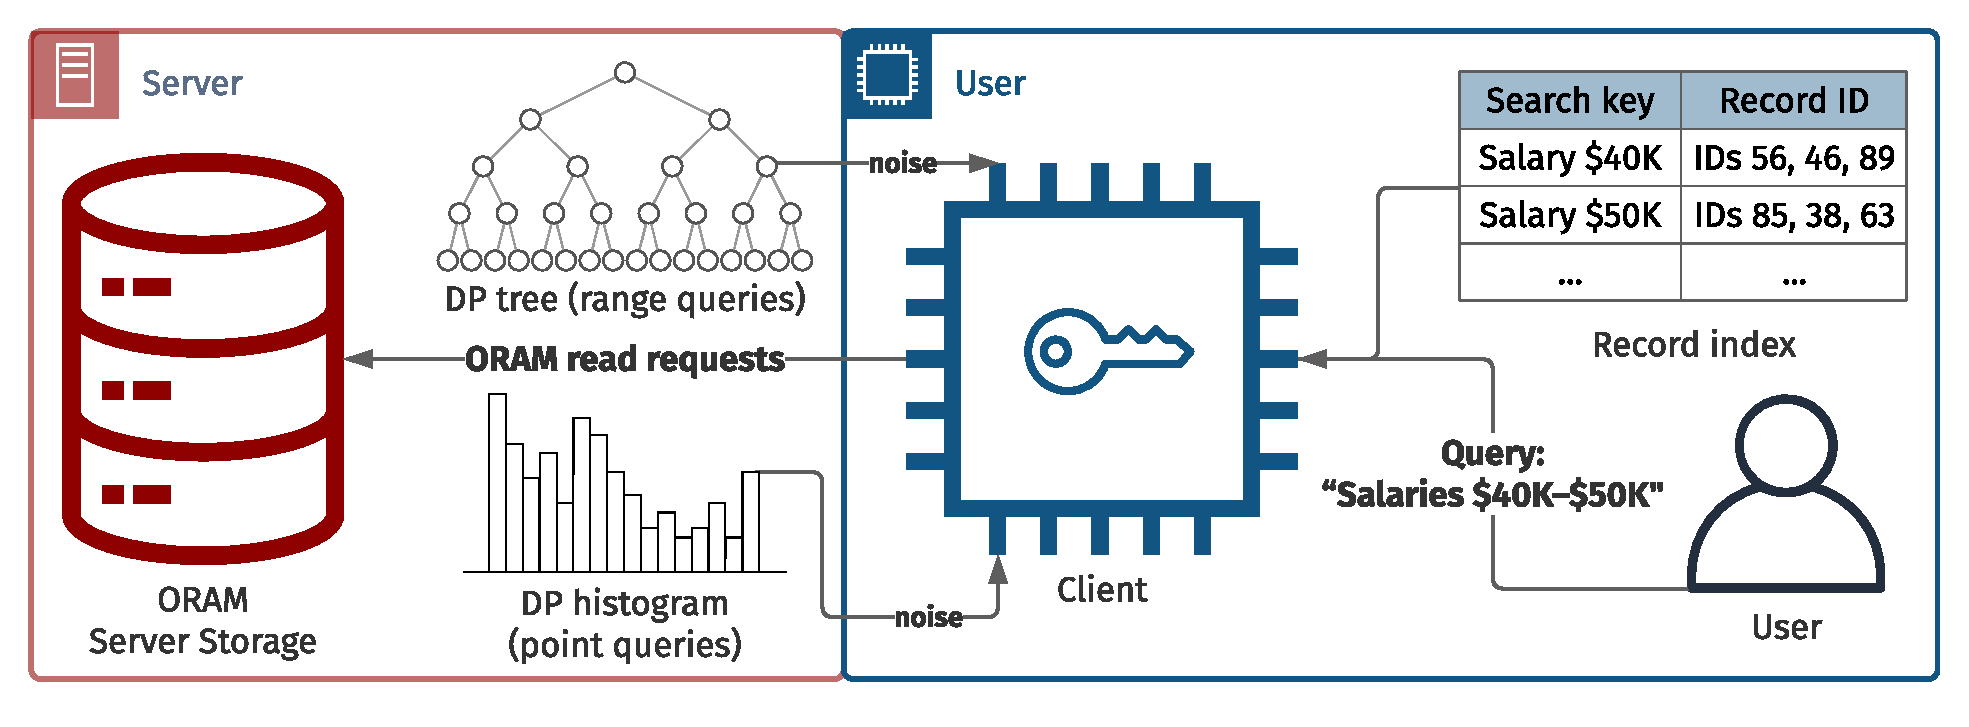
\includegraphics[width=\textwidth]{dp-oram}

		\end{block}

	\end{frame}

	\begin{frame}{Parallel \epsolute{}}

		\onslide<1->{
			\begin{itemize}
				\item
					Single-threaded version is prohibitively slow, must parallelize \\
					\begin{small}
						\indent{} Assume single-threaded solution generates $r$ real and $f$ fake records
					\end{small}

				\item Split \user{} and \server{} state into \oramsNumber{} ORAMs, run as separate machines
				\item Partition records randomly (by ID) into \oramsNumber{} partitions, generate \oramsNumber{} inverted indexes
				\item What to do about \serverDS{}?
			\end{itemize}
		}

		\begin{columns}[t]
			\begin{column}{0.5\textwidth}

				\onslide<2->{
					\begin{block}{\protocolSeparate{}: separate \serverDS{} per ORAM}

						\begin{itemize}[leftmargin=*]
							\item Composition of disjoint datasets: take max $\epsilon$
							\item Each ORAM incurs noise comparable to $f$
							\item Win by splitting ORAM work $r$ into \oramsNumber{} partitions and lose by multiplying noise $f$ times \oramsNumber{}
							\item That is, all ORAMs are processing $r + \oramsNumber f$ records in parallel
						\end{itemize}

					\end{block}
				}

			\end{column}

			\begin{column}{0.5\textwidth}

				\onslide<3->{
					\begin{block}{\protocolShared{}: shared \serverDS{} for all ORAMs}

						\begin{itemize}[leftmargin=*]
							\item Same number of total records per ORAM
							\item Generated noise is larger than $f$ (say, $\alpha f$)
							\item But it is split among \oramsNumber{} ORAMs
							\item That is, all ORAMs are processing $r + \alpha f$ records in parallel
						\end{itemize}

					\end{block}
				}

			\end{column}


		\end{columns}

		\onslide<4->{
			\begin{center}
				\textbf{\protocolShared{} wins if $\alpha < \oramsNumber$}, which it is for almost all values of \oramsNumber{} ($\oramsNumber \gtrapprox 4$)
			\end{center}
		}

	\end{frame}

	\begin{frame}{Parallel \epsolute{} diagram (with improvements)}

		\centering
		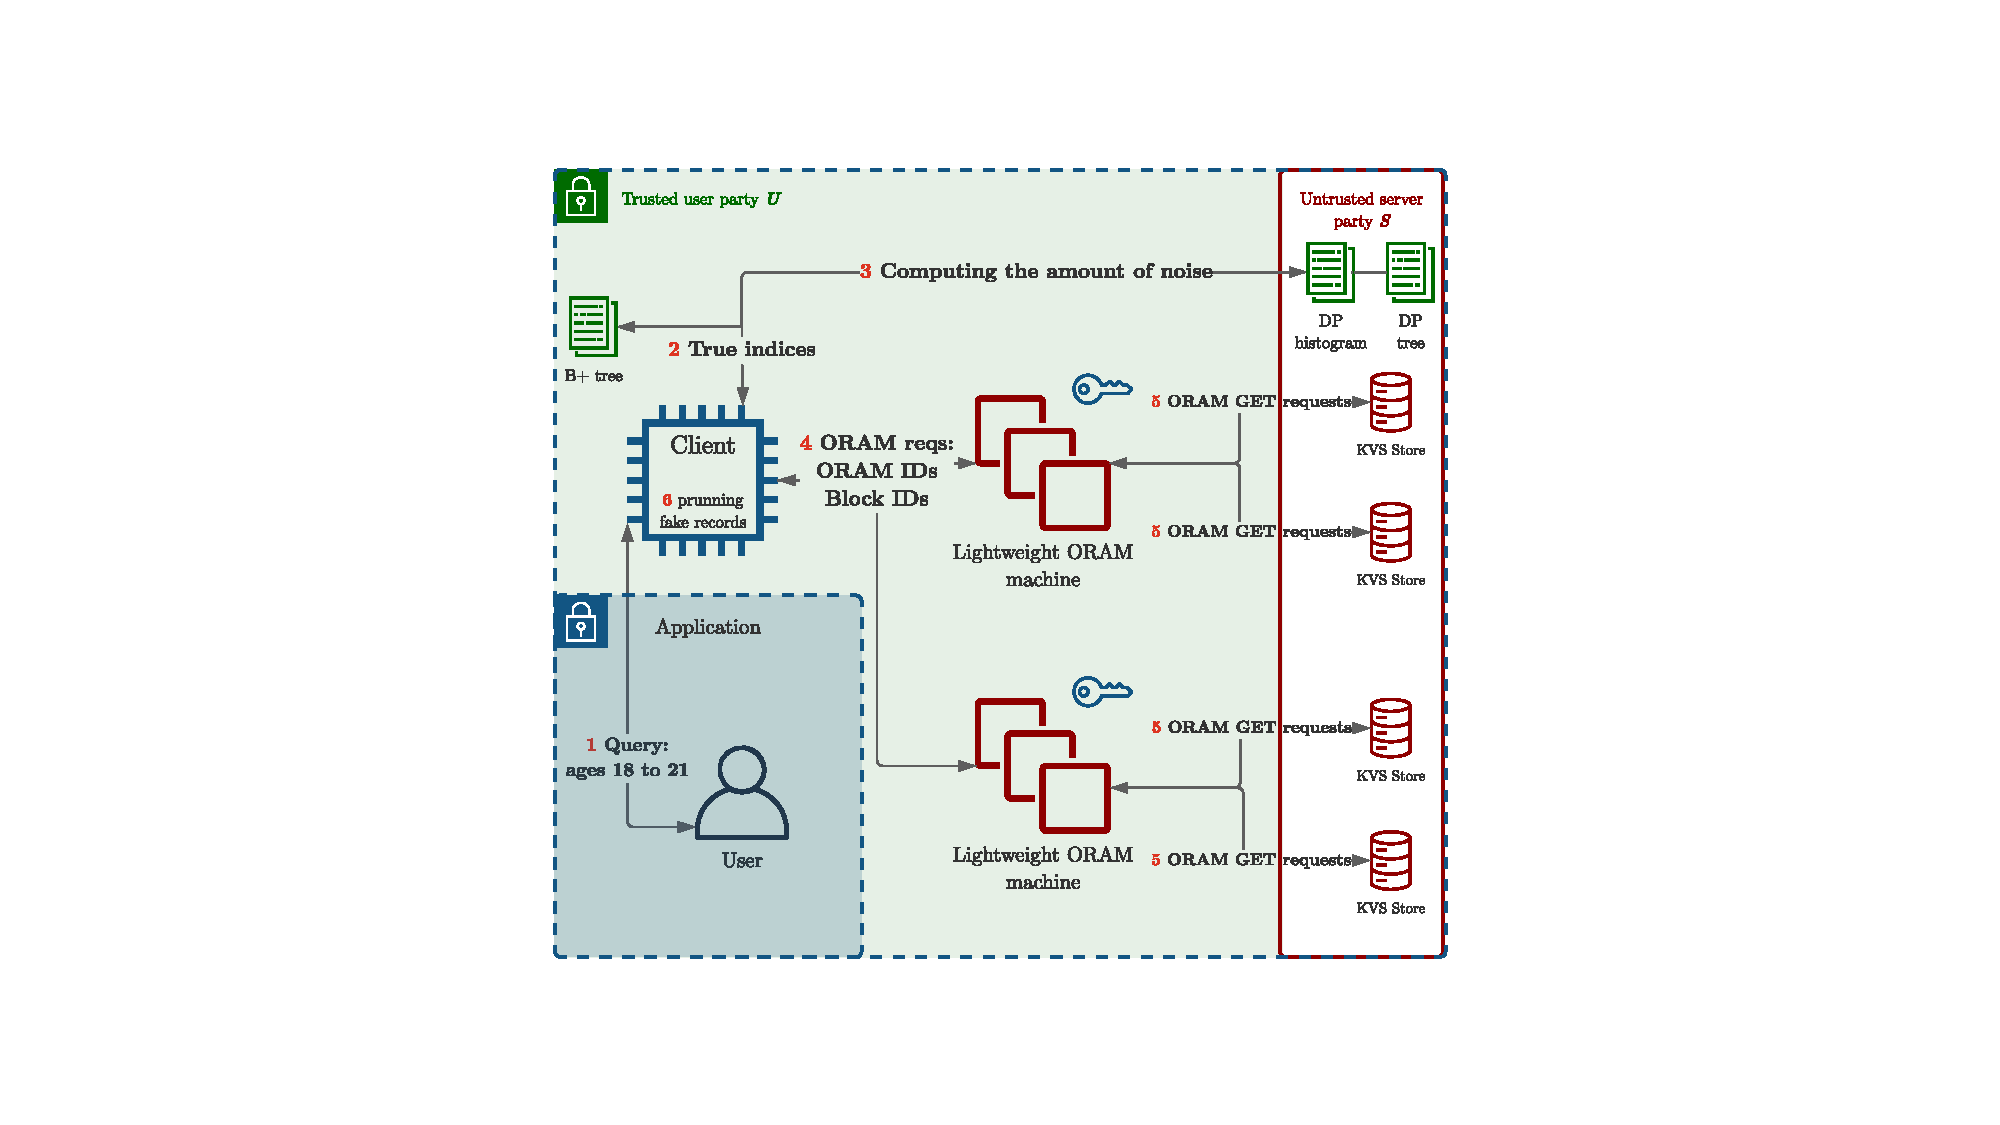
\includegraphics[width=0.63\textwidth]{three-layers}

	\end{frame}

	\begin{frame}{Experiments: scalability}

		\begin{figure}[h]
			\centering
			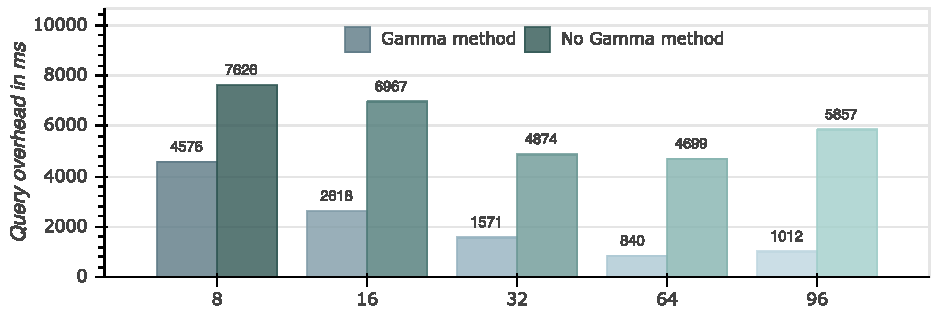
\includegraphics[width=\columnwidth]{scalability}
			\caption{Scalability measurements for \protocolShared{} and \protocolSeparate{}}%
		\end{figure}

	\end{frame}

	\begin{frame}{Experiments: against other mechanisms}

		\begin{figure}[h]
			\centering
			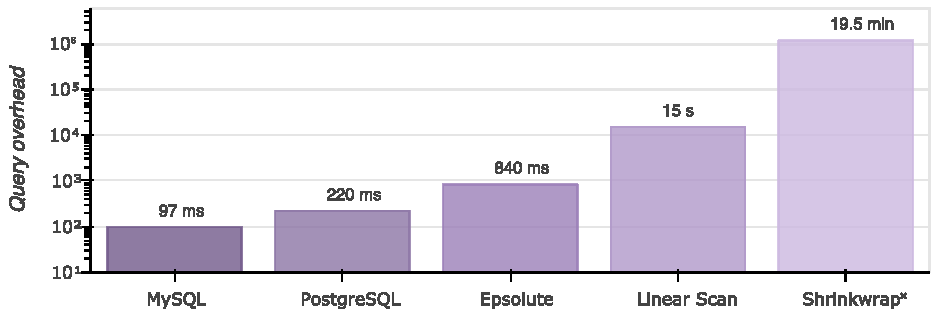
\includegraphics[width=\columnwidth]{mechanism}
			\caption{
				\centering
				Different range-query mechanisms (log scale). \ifthenelse{1=1}{\hspace{\textwidth}}{} % hack
				Default setting: $10^6$ \SI{4}{\kibi\byte} uniformly-sampled records with the range $10^4$.
			}%
		\end{figure}

	\end{frame}
